\documentclass[12pt]{beamer}
\usepackage[frenchb]{babel}
\usepackage[T1]{fontenc}
\usepackage[utf8x]{inputenc} 
\usepackage{ucs}   
\usepackage{graphicx}           % pictures
\usepackage{multimedia}         % sounds and movies
\usetheme{Warsaw}
\title {Projet Picross}
\author{Groupe B}
\date{16 Mai 2014}
\institute{Université du Maine}
%%%%%%%%%%%%%%%%%
% PREAMBULE     %
%%%%%%%%%%%%%%%%%
\setbeamertemplate{itemize item}[circle]
\hypersetup{
        pdfpagemode = FullScreen,% afficher le pdf en plein Ecran
        pdfauthor   = {groupe B},%
        pdftitle    = {projet}%
        pdfsubject  = {projet},%
        pdfcreator  = {PDFLaTeX},%
}
\setbeamertemplate{navigation symbols}{
        \insertslidenavigationsymbol
        \insertframenavigationsymbol
        \insertsubsectionnavigationsymbol
        \insertsectionnavigationsymbol
        \insertdocnavigationsymbol
        \insertbackfindforwardnavigationsymbol
}
% Faire apparaitre un sommaire avant chaque section
\AtBeginSection[]{
        \begin{frame}
        \begin{center}{\Large Plan }\end{center}
        %%% affiche en début de chaque section, les noms de sections et
        %%% noms de sous-sections de la section en cours.
        \tableofcontents[currentsection,hideothersubsections]
        \end{frame} 
}
%%%%%%%%%%%%%%%%%
% DOCUMENT      %
%%%%%%%%%%%%%%%%%
\begin{document}
\maketitle
% FRAME %%%%%%%%%%%%%%%%%%%%%%%%%%%%
\begin{frame}{}
  \tableofcontents
\end{frame}
   
%%%%%%%%%%%%%%%%%%
% Présentation
%%%%%%%%%%%%%%%%%%
\section{Présentation}
% FRAME %%%%%%%%%%%%%%%%%%%%%%%%%%%%
\begin{frame}
\frametitle{Présentation du Projet}
    \begin{enumerate}
     
      \item Présentation des membres
        \begin{enumerate}
        \item Lucas Bourneuf   (Chef de Projet)
        \item Ewen Cousin      (Developpeur GUI)
        \item Jaweed Parwany   (Developpeur Système)
        \item Charlie Marechal (Documentaliste)
        \item Nicolas Bourdin  (Developpeur GUI)
        \item Julien Le Gall    (Developpeur IA)
        \end{enumerate}\pause
     
      \item Objectif
        \begin{itemize}
            \item Créer un Picross en Ruby
        \end{itemize}\pause
     
      \item Delai
        \begin{itemize}
            \item 3 mois
        \end{itemize}
 \end{enumerate}   
 \end{frame}
    
   \begin{frame}
   \begin{enumerate}
   \item Liste des fonctionnalités
    
    \begin{enumerate}
                        
        \item Aide
        \begin{itemize}
            \item En cas de blocage on peut avoir accès à l'aide 
            \item Permet de trouver une solution selon deux niveaux
        \end{itemize}\pause
                        
        \item Gestion de sauvegarde
        \begin{itemize}
            \item Sauvegarde la partie dans un fichier
        \end{itemize}\pause
                        
        \item Score
        \begin{itemize}
            \item Affiche les scores de la grille en cours
        \end{itemize}\pause
                        
        \item Chargement de grille
        \begin{itemize}
            \item Permet le chargement d'une grille déjà crée
        \end{itemize}\pause
                        
        \item Edition
        \begin{itemize}
            \item Possibilité de créer ses propres grilles.
        \end{itemize}\pause
                        
        \item Manuel
        \begin{itemize}
            \item Affiche les règles du jeu
        \end{itemize}\pause
    \end{enumerate}
    
    
    \item Contraintes 
    \begin{enumerate}
        \item Temps
        \item Technique
    \end{enumerate}
    
    %\item "Il s'agit d'un picross blablabla"
    
    \end{enumerate}
\end{frame}


\section{Réalisation du projet}
\subsection{Le déroulement du projet}

\begin{frame}
\frametitle{Réalisation du projet}
 \begin{enumerate}
  \item Le déroulement du projet
    \begin{enumerate}
        \item Répartition des tâches
        \item Diagramme de Gantt
        \item Diagramme UML
    \end{enumerate}
 \end{enumerate}
\end{frame}


\begin{frame}
  \frametitle{Diagramme de Gantt}
  \begin{figure}[t]
    \centering
    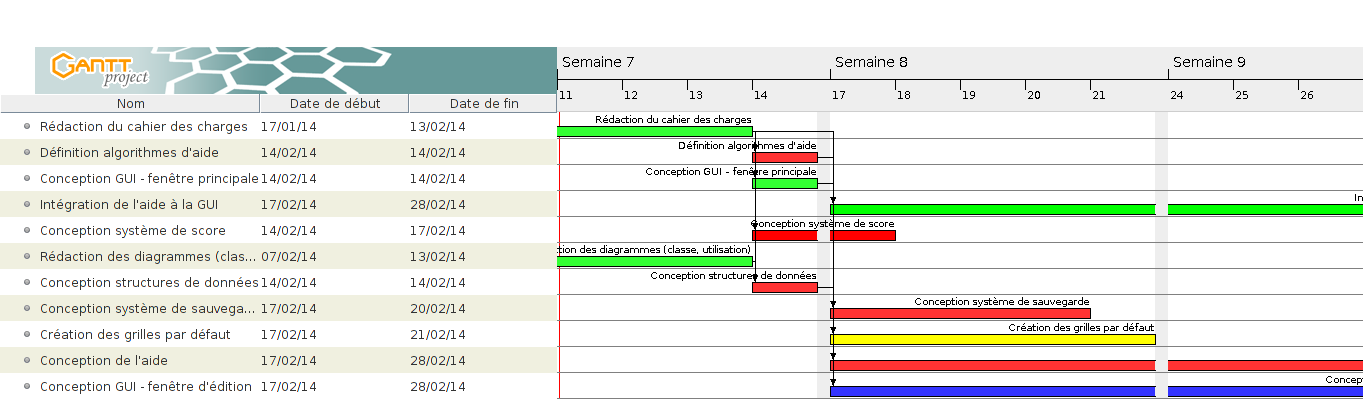
\includegraphics[scale=0.38]{ganttDiagram}
    \caption{Diagramme de Gantt}
  \end{figure}
\end{frame}

\begin{frame}
  \frametitle{Diagramme de UML}
  \begin{figure}[t]
    \centering
    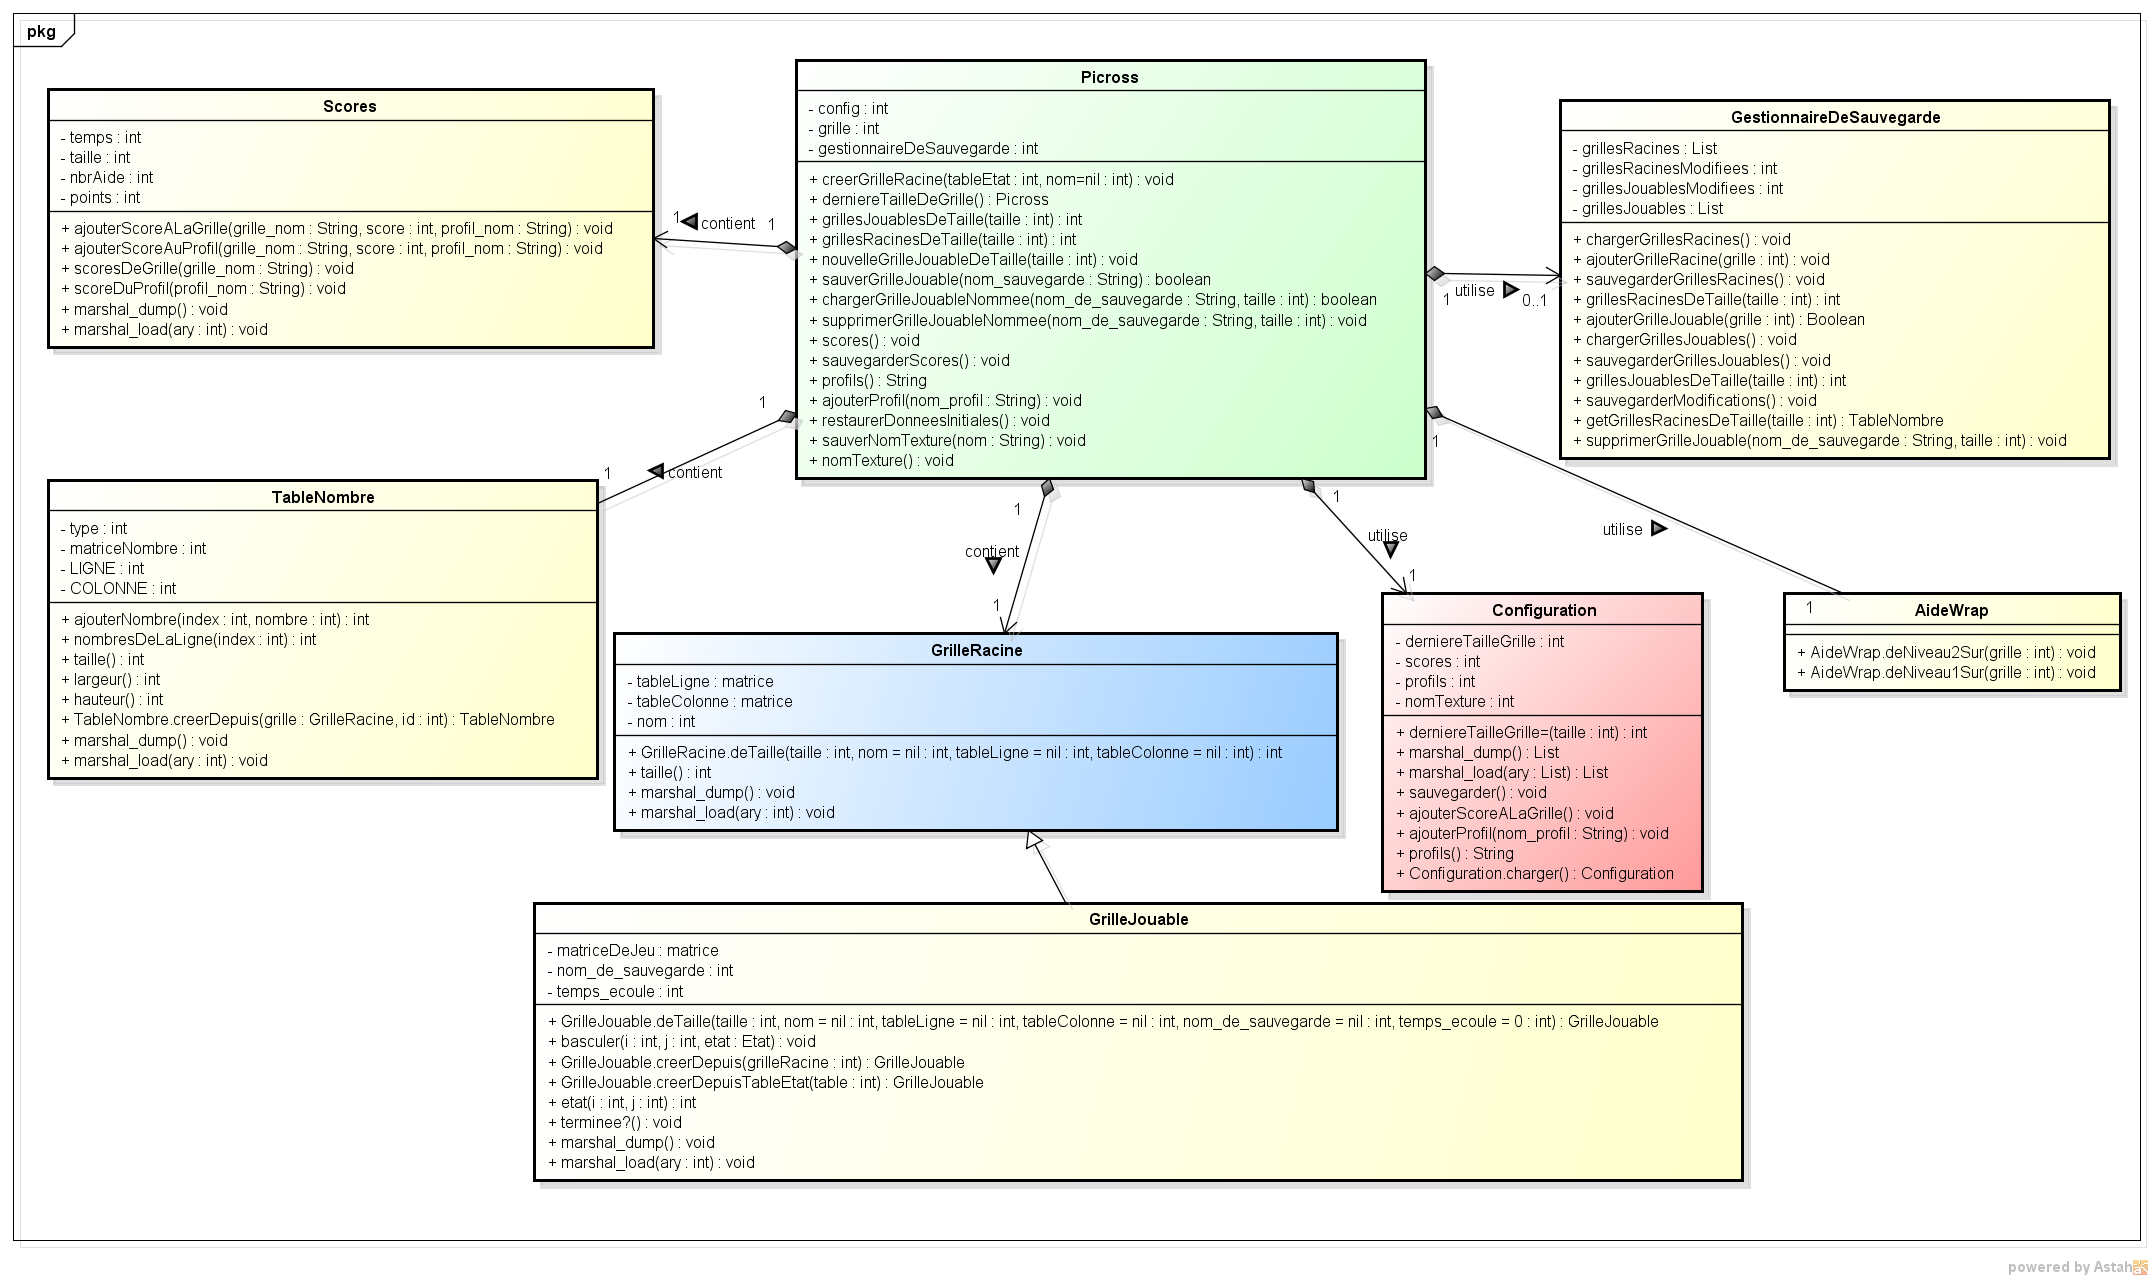
\includegraphics[height=\dimexpr11\textheight/16\relax]{UMLDiagram}
    \caption{Diagrammes UML}
  \end{figure}
\end{frame}

\subsection{Aspects techniques}
    \begin{frame}
    
        \begin{enumerate}
            \item Languages
            \begin{itemize}
                \item Ruby
                \item LateX
            \end{itemize}
                
            \item Support
            \begin{itemize}
                \item Environnement Unix
            \end{itemize}
                
            \item Outils
            \begin{itemize}
                \item IDE,
                \begin{itemize}
                    \item Vim,
                    \item kate,
                    \item sublim text,
                    \item textmate
                \end{itemize}
                \item Module RMagick
                \item IRC,
                \item Etherpad,
                \item Git/Github,
                \item GanttProject,
                \item Astah;
                    
            \end{itemize}
                
                    
        \end{enumerate}
\end{frame}


\subsection{Fonctionnalités}
    \begin{frame} 
    \frametitle{Fonctionnalités}
        \begin{enumerate}
            \item Fonctionnalités
            \begin{itemize}
                \item Drag 'n' assign
                \item Sauvegarde
                \item Chargement
                \item Edition
                \item Suppression
            \end{itemize}    
        \end{enumerate}
\end{frame}

\subsection{Difficultés}
    \begin{frame}
        \begin{itemize}
          \item Travailler en groupe, la répartition des taches
          \item Utilisation de github
        \end{itemize}
    \end{frame}

\section{Démo}
    \begin{frame}{Démo}
    \end{frame}

\section{Conclusion}
    \begin{frame}
    \frametitle{Conclusion}
        
        \begin{enumerate}
            \item Perspectives d'améliorations
            \begin{itemize}
                \item Statistique d'un profil
                \item Amélioration de l'interface 
            \end{itemize}
            
            \item Ce que l'on à appris
            \begin{enumerate}
                \item Comment un projet se déroule
                \item le travail collaboratif
            \end{enumerate}
            
            \item Ce que l'on a aimé
            
         
        \end{enumerate}
    \end{frame}
    
\appendix[Questions ?]
\end{document}
